\documentclass[11pt]{article}

\usepackage{graphicx}
\usepackage{hyperref}
\usepackage{fancybox}
\usepackage{pslatex}
\usepackage{mdframed}
\usepackage{xcolor}
\usepackage{caption}
\usepackage{subcaption}

\newcommand{\DCEC}{\ensuremath{\mathcal{DCEC}^\ast}}

\begin{document}

\title{Documentation for PAGI World: A Physically Realistic Simulation Environment for Developmental AI Systems}
\author{John Licato}
\maketitle

\begin{abstract}
This document is a partial documentation for getting started with PAGI World. It is by no means meant to be a complete tutorial, and may not make much sense to anyone who has not taken the EHLACS class with John Licato. We are working on a more complete tutorial and hope to complete it soon.
\end{abstract}

\tableofcontents

\section*{Update History}

\begin{itemize}
\item[10/10/14] Created document. \textit{---JL}
\end{itemize}

\section*{Known Bugs}

\begin{itemize}
\item none
\end{itemize}

\pagebreak

%\section{What is PAGI World?}q
%
%\section{Quickstart Guide}
%setting up a simple python script using the python library
%
%\section{Installing and Getting Started with PAGI World}
%
%\section{The PAGI World Environment}
%\label{sect:pagiEnvironment}
%objects and their basic properties
%loading and saving tasks
%all the menus
%
%\section{The PAGI Guy}
%body sensors
%tactile sensors
%hands
%visual field
%
%\section{Controlling PAGI Guy}
%controlling him through keyboard
%basic functions to control through code
%
%\section{Creating Your Own Tasks}
%\label{sect:creatingTasks}
%A full list of all the items available in the menu, and how they work
%
%\section{Sample Tasks}
%
%\section{Python Helper Library}
%
%
%\section{Advanced Development}

\pagebreak

\section{All Commands}

What follows is a list of all the possible commands that can be sent to PAGI World through TCP/IP. Every one of these should be terminated with an endline (\texttt{\textbackslash n}) character.

\subsection{Sensor Requests}

This is a complete listing of all sensors available, how to request their values, and what to expect in return.

\noindent \textbf{Command:} \texttt{sensorRequest,s} where \texttt{s} is the code of the sensor being requested. All sensor codes are listed below.

\subsubsection{Body tactile sensors}

For each of the body sensors (which are numbered 0 to 7), the sensor codes are \texttt{B0} - \texttt{B7}. The body is surrounded by these 8 sensors, which are placed at equal distances along the body's circumference. So in order to request the value of body sensor 5, you would send the string ``\texttt{sensorRequest,B5\textbackslash n}" (with no quotes).

\noindent \textbf{Returns:} A string of the form \texttt{s,p,tmp,tx1,tx2,tx3,tx4,e}, where:
\begin{itemize}
\item \texttt{s} - the sensor's code
\item \texttt{p} - 0 if the sensor detects nothing (in which case all following values will be 0), 1 if something was detected
\item \texttt{tmp} - The temperature value detected, as a float
\item \texttt{tx1-tx4} - The texture detected. This is four floats meant to describe the quality of the texture.
\item \texttt{e} - Body sensors only. This is the amount of "direct pleasure" the agent is currently feeling from that sensor. e.g., if the B0 sensor is touching a reward object, then this sensor will return a positive value for e. If it is touching a pain object, then it will return a negative value.
\end{itemize}
	
\subsubsection{Hand tactile sensors}

Each hand sensor has 5 tactile sensors, which are like the body sensors. The codes for the left hand's tactile sensors are \texttt{L0} - \texttt{L4}, while the right hand's tactile sensors have the codes \texttt{R0} - \texttt{R4}.

\noindent \textbf{Returns:} Same as the returned string for the body tactile sensors.

\subsubsection{Velocity sensors}

Tells you the current velocity of the body. Use sensor code \texttt{S}.

\noindent \textbf{Returns:}	 A string of the form \texttt{S,x,y}, where \texttt{x,y} are float values representing the x and y velocities of PAGI guy's body.

\subsubsection{Body position sensors}

Tells you the current absolute coordinates of the body. Use sensor code \texttt{BP}.

\noindent \textbf{Returns:} A string of the form \texttt{BP,x,y}, where \texttt{x,y} are float values representing the x and y coordinates of PAGI guy's body.


\subsubsection{Proprioception sensors}

Tells you the positions of the hands relative to the body. Use sensor code \texttt{LP} or \texttt{RP} for the left or right hands, respectively. Note that these are relative positions, so the proprioception coordinates of the hands will change relative to the rotation and position of the body.

\noindent \textbf{Returns:} A string of the form \texttt{s,x,y}, where \texttt{s} is the sensor code you sent, and \texttt{x,y} are float values representing the x and y coordinates of the hand relative to PAGI guy's body.

\subsubsection{Rotation sensor}

Tells you the current rotation of the body. Use sensor code \texttt{A}.

\noindent \textbf{Returns:} A string of the form \texttt{A,d} where \texttt{d} is the current rotation of the body in radians.

\subsubsection{Vision sensors}

There are two categories of vision sensors, the \textit{detailed} and the \textit{peripheral} vision sensors. The detailed vision sensors, whose sensor codes are \texttt{V0.0 - V30.20}, are located at intervals of 0.15 world coordinate units (approximately 15 pixels), measured from the bottom-left corner of the detailed visual field. For example, V4.7 is the visual sensor that is located 4x15=60 pixels to the right of sensor V0.0, and 7x15=105 pixels above. V30.20 is on the top-right corner of the visual field.

The peripheral visual sensors, whose sensor codes are \texttt{P0.0 - P15.10}, are located at 0.667 world coordinate units (approximately 66.7 pixels), measured from the bottom-left corner of the peripheral visual field. For example, P4.7 is the visual sensor located 4x66.7=267 pixels to the right of sensor P0.0, and 467 pixels above.

\textit{Simple mode} is turned on by default, and simply means that more information is given by the visual sensors. Currently, simple mode cannot be turned off.

\noindent \textbf{Returns:} A string of the form \texttt{s,vq1,vq2,vq3,v4,[,t,n]} where:

\begin{itemize}
\item \texttt{s} - the vision sensor's code
\item \texttt{vq1-vq4} - floats which capture the visual description by the sensor. This will correspond to things like color, fuzziness, etc. currently just returns 0 for each.
\item \texttt{t} - [only in simple mode] a string describing the type/category of the object, e.g. ``chair" or ``human".
\item \texttt{n} - [only in simple mode] a string of the unique id of the object, e.g. ``chair121" or ``Bob".
\end{itemize}

\subsubsection{Map vision sensors}

Sometimes you will find it too slow to request single sensor values at a time, and will need to download the entire visual field in one shot. There are two commands available for this. Sensor code \texttt{MDN} returns the data from the detailed sensors, and \texttt{MPN} does the same for the peripheral sensors. 

\noindent \textbf{Returns:} A string of the form \texttt{s,n0.0,n1.0,...} where \texttt{s} is either \texttt{MDN} or \texttt{MPN}, depending on which command you sent. Each \texttt{nx,y} is the name/unique id of the object seen by the sensor. If no object was seen by that sensor, then it is an empty string (so you'll see two commas with nothing in between). The values are sent in row-major order, so for example with detailed visual sensors the order will be \texttt{n0.0, n1.0, n2.0, \ldots, n30.0, n0.1, n1.1, \ldots, n30.20}.

\subsubsection{Object searches}

Although it is not quite low-level, the option is also provided to do a search within the visual field for an object of a specific name. This is done by sending the special command (note this is not a sensor request) \texttt{findObj,objName,searchMode}, where \texttt{objName} is the name of the object you are searching for. \texttt{searchMode} describes the options for the search, which are either \texttt{P} for peripheral visual sensors only, \texttt{D} for detailed visual sensors only, and \texttt{PD} for both.

\noindent \textbf{Returns:} A string of the form \texttt{findObj,objName[,s1][,s2]...} where:

\begin{itemize}
\item \texttt{objName} - the name of the object being searched for (see below)
\item \texttt{si} - the visual sensor at which the object was found. 
\end{itemize}

Although this is not a complete list of all the possible \texttt{objName} values (since it will be updated frequently), let this serve as a partial guide:

\begin{itemize}
\item Ramps: \texttt{rightRamp, leftRamp, floatingRightRamp, floatingLeftRamp}
\item Wall and block pieces: \texttt{wallBlock, horizontalWall, verticalWall, floatingWallBlock, floatingHorizontalWall, floatingVerticalWall, iceBlock, lavaBlock, blueWall, greenWall, redWall}
\item Dynamite: \texttt{redDynamite, greenDynamite, blueDynamite}
\item Rewards/Punishments: \texttt{apple, bacon, redPill, bluePill, poison, steak}
\item Other: \texttt{soldier, medkit}
\end{itemize}


\subsection{Force Effectors}

Force effectors allow you to essentially control PAGI guy's movement. In keeping with the philosophy of PAGI World, you don't move PAGI guy directly; rather you can send forces in particular directions. For example, to move one of his hands downwards, you send a downward force to the hand, and this will exert an equal and opposite force on his body. With enough force, you can even get him to push downwards with his hands to get him to ``stand up" using his arms as legs!

All force effector commands are of the form: \texttt{addForce,e,v} where \texttt{e} is the effector code, and \texttt{v} is the amount of force to be sent (this is necessary for all but ignored by some effector codes, see the descriptions that follow). All effector codes return a string of the form \texttt{e,1} if the force was successfully applied, or \texttt{e,0} if there was an error, where \texttt{e} is the effector code that was sent.

You can replace \texttt{v} with a basic arithmetic expression. To do this, wrap it in square brackets. Expressions can contain the basic arithmetic operators ($+$, $-$, $/$, and $*$), float values, and sensor aspect codes (Section \ref{sect:sensorAspectCodes}). So for example, if you want to send a force to the body to move vertically, where the force is equal to twice the y coordinate of the body, you would use:

\texttt{addForce,BMV,[2*BPy]}

\subsubsection{Hand and body forces}

To apply forces to the left hand, use effector codes \texttt{LHV} and \texttt{LHH}, for vertical and horizontal movement respectively. \texttt{v} can be positive or negative. Likewise, to move the right hand use \texttt{RHV} or \texttt{RHH}, and for the body use \texttt{BMV} and \texttt{BMH}. Currently you are allowed to add arbitrary force in the up/down directions, so effectively you can make him fly. But this is likely to be removed in later versions, so try to avoid using it!

You also have the option of sending vertical and horizontal movements in one command. Use effector codes \texttt{LHvec}, \texttt{RHvec}, and \texttt{BMvec} for the left hand, right hand, and body respectively. For example, if you want to send a force vector to the right hand of 3.1 in the x direction and 2.0 in the y direction, you'd use the command:

\texttt{addForce,RHvec,3.1,2.0}

\subsubsection{Jumping}

Use effector code \texttt{J} to make PAGI guy jump. Use a force of about 30,000 for a good jump. A jump will also exert an equivalent downward force on whatever object the bottom of the body was touching at the time of the jump. If the bottom of the body is not touching anything, the jump will not be carried out and \texttt{J,0} will be returned.

\subsubsection{Rotation}

To rotate the body, use effector code \texttt{BR}. \texttt{v} is the amount of torque to use to rotate the body (can be positive or negative).

\subsubsection{Gripping and releasing}

To have the hands grip or release, send the relevant effector codes with \texttt{v} set to 0 (\texttt{v} is ignored here). To make the right or left hand grip, use effector codes \texttt{RHG} and \texttt{LHG} respectively. To make the right or left hands release, use effector codes \texttt{RHR} or \texttt{LHR}. A hand is in a gripping state until it is sent a command to release.

\subsection{States and Reflexes}
\label{sect:statesAndReflexes}

Although TCP/IP communication is normally quite fast, there are some times when you will need PAGI guy to react much quicker, or to notify the AI side when a certain combination of sensors is met. For this reason, a \textit{states and reflexes} system is built into PAGI World. Setting reflexes involves the most complex commands available within PAGI World, and \textbf{this section is only recommended for advanced users who have exhausted the means available in the other sections.}

A \textit{state} in PAGI World is in a simple binary state: it is either active, or it is not. To establish a state, send a command of the form \texttt{setState,s,d} where \texttt{s} is the unique name of this state, and \texttt{d} is the duration that this state will remain active, measured in milliseconds. If you want a state to remain active indefinitely, set \texttt{d} to -1. If you want to remove, or deactivate a state, set \texttt{d} to 0.

A \textit{reflex} in PAGI World allows PAGI guy to automatically respond to a certain state of the world automatically, much faster than if this were dependent on TCP/IP. However, we do not recommend making your program reflex-heavy; reflexes should be reserved for those actions that require precisely timed or incredibly quick actions. To create a reflex, send a command of the form \texttt{setReflex,n,C[,A]} where:

\begin{itemize}
\item \texttt{n} - The unique name of this reflex. If a reflex with this name already exists, this will replace the older reflex.
\item \texttt{C} - A listing, where each item is separated by a semicolon, of the conditions that must be met for this reflex to be triggered. There are two types of conditions: state conditions, and sensory conditions. 
	\begin{itemize}
	\item \textbf{State conditions} simply are used to check if a state is active or not. Each state condition is of the form \texttt{[-]s} where \texttt{s} is simply the name of the state. The hyphen, which is optional, makes it so that the condition is only satisfied if the state \texttt{s} is \textit{not} active.
	\item \textbf{Sensory conditions} are met if a particular sensor aspect has a value that is above, below, or equal to a certain value. Sensor aspects are the float values that are associated with each sensor. For example, each of the hand sensors checks for temperature, a four-dimensional texture vector, and endorphins. Here the temperature value, the endorphin value, and each of the four floats making up the texture vector are all sensor aspects. Each of these sensor aspects has a unique code which is listed below.\\
	Each sensory condition is of the form \texttt{q|o|v} where \texttt{q} is the code of the sensor aspect (see Section \ref{sect:sensorAspectCodes}), \texttt{o} is the operator to use to compare (which is either $<, >, =,$ \{ for $\leq$, \} for $\geq$, or ! for $\neq$) and \texttt{v} is the value to use. For example, \texttt{L0\_tx1|\{|0.1} means that we want to check the first float of the texture vector detected by left hand sensor 0. If it is less than or equal to 0.1, then this sensory condition is satisfied. For the equality operator ($=$), there is a tolerance of 0.01, so that for the expression \texttt{L0\_tx1|$=$|5.0}, any values of \texttt{L0\_tx1} from 4.9 to 5.1 will be accepted.
	\end{itemize}
\item \texttt{A} - (optional) A listing, where each item is separated by a semicolon, of the actions to be executed if every condition in \texttt{C} is met. Each action is another command, except for another reflex command, with all of the commas replaced by the pipe character (\texttt{|}).
\end{itemize}

Here's an example which makes use of the states and reflexes system. Let's say that you defined a state called ``\texttt{testState}". If \texttt{testState} is active, you want a reflex to fire that will have two actions take place: You want PAGI guy to move right, and you want him to jump. Normally the commands for these actions would be \texttt{addForce,BMH,100} and \texttt{addForce,J,30000} respectively. In order to create this reflex, you would use:

\noindent \texttt{setReflex, testReflex, testState, addForce|BMH|100;addForce|J|30000}

Now let's say you wanted to add another reflex that has two conditions: the downward velocity of PAGI guy's body has to be greater than 100 (\texttt{Sx|>|100}), and the state \texttt{testState} must be active. You want it to have zero actions (this is sometimes useful when you only want the notification that the conditions were met). You would use the command:

\noindent \texttt{setReflex, testReflex2, testState;Sx|>|100 }

\subsubsection{Other state and reflex commands}

To remove a state, send the command \texttt{setState,s,0} where \texttt{s} is the name of the state you want to disable.

To remove a reflex, simply send the command \texttt{removeReflex,n} where \texttt{n} is the name of the reflex to remove.

You can get a listing of all active states with the command \texttt{getActiveStates}. It returns a string of the form \texttt{activeStates,s1,s2,...} where each \texttt{si} is the name of a state that is currently active. 

To get a listing of all active reflexes, use the command \texttt{getActiveReflexes}. It returns a string of the form \texttt{activeReflexes,r1,r2,...} where each \texttt{ri} is the name of a reflex that is currently active.

\subsubsection{All sensor aspect codes}
\label{sect:sensorAspectCodes}

L0\_tmp - Left hand sensor 0 temperature\\
L0\_tx1 - Left hand sensor 0 texture vector component 1\\
L0\_tx2 - Left hand sensor 0 texture vector component 2\\
L0\_tx3 - Left hand sensor 0 texture vector component 3\\
L0\_tx4 - Left hand sensor 0 texture vector component 4\\
L0\_e - Left hand sensor 0 endorphins\\
\textit{Likewise for L1 through L4, R0 through R5 for the right hand, and B0 through B7 for the body's tactile sensors. Simply replace `L0' with the appropriate sensor code.}

\noindent Sx - x velocity of body\\
Sy - y velocity of body\\
BPx - absolute x coordinate of body\\
BPy - absolute y coordinate of body\\
LPx - x coordinate of left hand relative to body\\
LPy - y coordinate of left hand relative to body\\
RPx - x coordinate of right hand relative to body\\
RPy - y coordinate of right hand relative to body\\
A - rotation of the body in radians

\noindent V0.0\_vq1 - Detailed visual sensor description vector component 1\\
V0.0\_vq2 - Detailed visual sensor description vector component 2\\
V0.0\_vq3 - Detailed visual sensor description vector component 3\\
V0.0\_vq4 - Detailed visual sensor description vector component 4\\
\textit{Likewise for V0.1 through V30.20 for the detailed visual sensors, and P0.0 through P15.10 for the peripheral visual sensors.}





\subsection{Creating Items Dynamically}

Through commands, you can create items in real-time.

\subsubsection{Creating Menu Items Dynamically}

Some items can be created during runtime by sending commands from the AI side. Simply send a command of the form \texttt{dropItem,n,x,y[,n]}, where:

\begin{itemize}
\item \texttt{n} - The object name of the item to generate.
\item \texttt{x,y} - The x,y positions where the item should initially appear.
\item \texttt{n} - an additional note (usually optional, but required for some item types. See item codes below for more details. If the item type doesn't require this, it is ignored.)
\end{itemize}

The object names are the same identifiers that are returned by sensors, e.g. the \texttt{objName} field in the \texttt{findObj} command.

\subsubsection{Creating and Controlling Custom Objects}

(As of version 0.1.7) It is possible to create your own objects in PAGI World, which you can then control by sending force commands. This is done by calling the command:

\texttt{createItem,name,fp,x,y,m,ph,r,e,d,k} where:

\begin{itemize}
\item \texttt{fp} - The path to the image to be used. The image must be either a png, jpg, or jpeg. The filename must have no commas or this string will be messed up! Also note that the image file is \textit{not} saved with task files, so if you have a task file that has custom items, use relative directories and always include the image files with your task files. The image will be loaded at a size of 50 pixels per world unit. Also, the size of the bounding box will \textit{always} be rectangular, regardless of the shape of the image. You may load png files if you want partially transparent images, but the bounding box will still be calculated based on the total image size.
\item \texttt{name} - The unique string identifier for this individual item. If you use a name that is already taken, then the previous item with this name will be deleted.
\item \texttt{x,y} - The x,y positions where the item should initially appear.
\item \texttt{m} - The initial mass of the item. For reference, the mass of an apple is 1, and the mass of a wall piece is 50.
\item \texttt{ph} - The physics material to use for this item. This can be one of the following:
	\begin{itemize}
	\item 0 - Low friction, low bounciness
	\item 1 - Normal friction, low bounciness (Most items should be this setting by default)
	\item 2 - High friction, low bounciness
	\item 3 - Low friction, high bounciness
	\item 4 - Normal friction, high bounciness
	\item 5 - High friction, high bounciness
	\end{itemize}
\item \texttt{r} - The initial rotation of the item, in radians. 
\item \texttt{e} - The amount of endorphins the object provides.
\item \texttt{d} - 1 if the object should disappear upon contact with PAGI guy (e.g., if it is a food or poison item), 0 otherwise.
\item \texttt{k} - Kinematic properties of the item. An object can be kinematic (meaning it will not move or rotate), fixed angle (meaning it will move but not rotate), and backgrounded (meaning it will not interact with other items in the world). The value you send for \texttt{k} will determine which combination of properties the object has:
	\begin{itemize}
	\item 0 - Kinematic, and backgrounded (kinematic automatically implies fixed angle).
	\item 1 - Kinematic, and not backgrounded. 
	\item 2 - Not kinematic, fixed angle, and backgrounded.
	\item 3 - Not kinematic, fixed angle, and not backgrounded.
	\item 4 - Not kinematic, not fixed angle, and backgrounded.
	\item 5 - Not kinematic, not fixed angle, and not backgrounded (the vast majority of items in the world will be this setting).
	\end{itemize}
\end{itemize}

After an item has been created, you can send force commands to it using:

\texttt{addForceToItem,name,fx,fy,fa} where:

\begin{itemize}
\item \texttt{name} - The unique name you gave to this item when you first created it. Errors will be returned if the name is not found (which might happen if the object was destroyed.
\item \texttt{fx,fy} - The amount of force in the horizontal and vertical directions (NOT relative to the item's rotation)
\item \texttt{fa} - The amount of rotational force to send to this item.
\end{itemize}

You are very strongly encouraged to send forces to custom created items to avoid unexpected behavior with PAGI World's physics engine. %Note that there are NO ways to directly set the positions or velocities of created items. This is to discourage any sort of perceptual input about things in the world that are not obtained through PAGI guy's sensors.
To get information about an item, call:

\texttt{getInfoAboutItem,name} where \texttt{name} is the unique name of this item. This will return an error message if the item was deleted or the name was not found. Otherwise, this command will return:

\noindent \textbf{Returns:} A string of the form \texttt{getInfoAboutItem,name,px,py,vx,vy} where:

\begin{itemize}
\item \texttt{name} - The name of the item
\item \texttt{px,py} - The x and y coordinates of the item
\item \texttt{vx,vy} - The x and y velocities of the item
\end{itemize}

Frequent use of \texttt{getInfoAboutItem} is \textbf{strongly discouraged}, as using any sort of perceptual input about things in the world that are not obtained through PAGI guy's sensors is against the intention of PAGI World. Do not get too attached to this command---future versions may severely limit its use somehow or remove it entirely!

You can also destroy custom created items, by calling:

\texttt{destroyItem,name} where \texttt{name} is the unique name of this item. 

\subsection{Others}

\subsubsection{Loading Tasks / Resetting Tasks}

In order to load a new task, or to reset the current task (assuming it is saved as a .TSK file), use the command:

\texttt{loadTask,f}

\noindent where \texttt{f} is a file path of a TSK file. To create TSK files, just press tab while PAGI World is loaded, and you can save the current task.

\subsubsection{Printing Text to the Screen}

To display text in the PAGI World console (obtained by pressing the ``backquote'' key, usually the same key that contains the tilde (~)), use the \texttt{print} command:

\texttt{print,S}

\noindent where \texttt{S} is the string to print. Note that everything in S is printed until the end-of-line character is reached. So if you were to send the command \texttt{print,this is a test, so is ``this''}, the console will display:

\texttt{AI-side says: this is a test, so is ``this''}

\subsection{Unprovoked Notifications}

There are many messages that may be sent from PAGI World to the AI side that are related to events that happened in the world which may not have been directly triggered by the AI side. For example, if a \textit{trigger box} is activated, a message will be sent to the user. Likewise if a reflex is activated (see Section \ref{sect:statesAndReflexes} for information on those notifications).

\subsubsection{Endorphins: Rewards and Punishments}

The basic reward / punishment system utilized by PAGI World is the \textit{endorphin}, which is a property of items in the environment. If an item which has a nonzero endorphin value touches the body, a message of the form \texttt{RD,e,l} is sent to the AI side, where \texttt{e} is the endorphin value (positive is good, whereas negative is bad), and \texttt{l} is the location on the body which is reporting contact with the endorphin, which ranges from 0-7 depending on which body sensor was closest.

\subsubsection{Spoken commands}

PAGI World can also ``hear" commands in plain text which are given to it by the environment. Currently the only way to do this is to type a message in the command box, which can be made visible through one of the menus (see Section \ref{sect:pagiEnvironment}). The command received is of the form \texttt{SC,x}, where \texttt{x} is the string which was sent through the command box.

\subsubsection{Triggers}

One of the items that can be created using PAGI World's task creator is a \textit{trigger box}, which is essentially a rectangular region of the environment that does not interact with the rest of the world in any physical way. The trigger boxes can be configured to fire if PAGI guy performs certain actions while within the box's boundaries (see Section \ref{sect:creatingTasks}). This will trigger a message to be sent to the AI side of the form \texttt{TB,n,c} where \texttt{n} is the name of the trigger box, and \texttt{c} is the action that the box detected within its boundaries. The possible values for \texttt{c} are:

\begin{itemize}
\item{LE/LX} - Left hand entered or exited the box, respectively
\item{RE/RX} - Right hand entered or exited the box, respectively
\item{BE/BX} - Body entered or exited the box, respectively
\item{RG/RR} - Right hand gripped or released its grip in the box, respectively
\item{LG/LR} - Left hand gripped or released its grip in the box, respectively
\item{OE/OX} - Another object (not a hand or the body) entered or exited the box, respectively
\end{itemize}

\textit{Note:} Remember that the trigger box must be configured to fire on each event type that you want it to watch for!
	


%\section{Introduction}
\label{sect:introduction}

Towards the end of his long and extremely distinguished career, Jean Piaget began to name and concretely describe some mechanisms which he believed were responsible for the emergence of many features of mature cognition: formal reasoning, an understanding of causality, and analogical ability were among these, along with many others \cite{Piaget1958,Piaget1974,Piaget2001}.
Piaget had long suspected that these features and the concepts they relied on were constructed by the child using simpler schemas acquired through interaction with the physical world, at least since Piaget and Inhelder (1958). Thus the role that the world plays in shaping the constructs and abilities of the child, which informs the related question of how much AI can progress without having a real-world-like environment, has been a cornerstone issue of AI for some time now \cite{Brooks1990,Brooks1991,Harnad1990}.

But modeling Piaget's beliefs is, to this day, an unmet goal. This is a dream of computational cognitive modelers, but perhaps more specifically the field of developmental AI---This is the field which attempts to show how, using an agent endowed with minimal innate capacities embedded in a sufficiently rich environment, higher-level cognitive abilities can emerge. These abilities may include logico-mathematical reasoning, an understanding of causality, robust analogical reasoning, and others. Furthermore, work in developmental AI systems has strived to show that the emergence of such abilities could be done in such a way that reflects the way they develop in humans, whether this is in the pattern predicted by Piaget's stage theories, Neo-Piagetian stage theories, or more gradually.

Frank Guerin (2011), in his recent survey of the Developmental AI field, concluded that current systems were lacking in several key areas\nocite{Guerin2011}. Guerin then suggested that a major reason (arguably the most important reason) why the field has the shortcomings he described, was the absence of a suitable simulation environment. Current simulation environments used by Developmental AI projects were missing several key features, and Guerin described some conditions that would need to be met by simulation environments in order to cure this problem. Among the most important of these are the following, which we refer to as \textbf{C1}, \textbf{C2}, and \textbf{C3}:

\begin{itemize}

\item[\textbf{C1}] It is rich enough to provide knowledge which would bootstrap the understandings of concepts rooted in physical relationships, e.g.: inside vs. outside, large vs. strong, etc.

\item[\textbf{C2}] It can allow for the modeling and acquisition of spatial knowledge, which Guerin notes is widely regarded to be a foundational domain of knowledge acquisition, through interaction with the world.

\item[\textbf{C3}] It can support the creation and maintenance of knowledge which the agent can verify itself.

\end{itemize}

This paper describes a task-centered, physically realistic simulation environment that we have developed to simultaneously address challenges \textbf{C1-C3}. By doing so, it is our hope that this system can remove a glaring roadblock in the fields of developmental AI and cognitive modeling in general. The plan for this paper is as follows: we will elaborate on conditions \textbf{C1-C3}, and close out this section by explaining the concepts of PAI and PAGI. Section \ref{sect:PAGI_World} attempts to answer why such a simulation environment does not currently exist, and then fully introduces PAGI World. Section \ref{sect:example_tasks} outlines several examples of tasks in PAGI World and AI solutions we developed to perform some of these tasks. Next, Section \ref{sect:criticisms} tries to respond to any possible objections to the assumptions and claims we make in this paper. Finally, we conclude and discuss exciting next steps.

\subsection{Guerin's Conditions}

A common theme running through conditions \textbf{C1-C3} is that what is lacking from current microworlds is a physically realistic environment---one in which the agent can acquire, develop, and test its concepts. But the concerns raised by Guerin (2011) are not only of interest to the field of Developmental AI; in fact all of AI in general can benefit by addressing them. For example, feature \textbf{C1} is extremely important for cognitive models of analogy, which are currently struggling to overcome what has been called the Tailorability Concern (TC)\cite{Gentner2011,Licato2013b}. The TC, brutally summarized, is that models of analogy (though this can be applied to all cognitive architectures in general) have far too long dealt almost exclusively with manually constructed knowledge representations, using toy examples often selected solely to display some particular ability. Licato et al. (2013) goes on to argue that overcoming the TC is necessary to progress the fields of analogy and cognitive architectures. After making this point, they develop a set of conditions that must be met in order to claim victory over the TC:

%\begin{mdframed}[skipabove=0.05in,skipbelow=0.1in,roundcorner=10pt,backgroundcolor=gray!15,
%  linewidth=0pt,roundcorner=8pt,fontcolor = black!90,
%  frametitle={ $TCA_3$ }
%    ,frametitlerule=true,frametitlerulecolor=gray!80,
%  frametitlebackgroundcolor=gray!30, frametitlerulewidth=0.5pt]
%\begin{itemize}\begin{footnotesize} \itemsep0pt
%\item A set of justificatio
%\end{footnotesize}
%\end{itemize} 
%\end{mdframed}

\begin{small}
\begin{quote}
\begin{mdframed}[backgroundcolor=gray!15]
$\mathbf{TCA_3}$ A computational system of analogy answers the TC if and only if given no more than either
\begin{itemize}
\item unstructured textural and/or visual data, or
\item a large, pre-existing database,
\end{itemize}
and minimal input, it is able to consistently produce \textit{useful} analogies and demonstrate stability through a variety of input forms and domains.
\end{mdframed}
\end{quote}
\end{small}

According to $\mathbf{TCA_3}$, then, good performance by the part of a cognitive agent on a sufficiently large knowledge base from which source analogs could be drawn is required to answer the TC. An agent interacting in the sort of microworld called for by Guerin (2011) might ideally be able to acquire such source analogs by simply interacting with its environment. 

\textbf{C1} and the TC together require that the microworld itself is what provides the knowledge which is drawn upon to construct concepts of basic physical relationships, not manually constructed source analogs or fully explicit logical theories. \textbf{C2} expands on \textbf{C1} by requiring that this knowledge of physical relationships not be static, but rather should allow for an agent in the world to learn through interaction. The idea that children learn by initiating interactions with the world based on their (often incomplete) conceptions of reality---in a manner that resembles scientific experimentation---was championed by Piaget and later constructivists \cite{vonGlasersfeld1991,Quartz1997,Piaget2001b}, and is at the core of views like the Bickhard's Interactivist Model \cite{Bickhard2008}.

A microworld that meets \textbf{C2}, then, should recognize that the concepts, schemas, and representations used by the agents will frequently change, and this is difficult to do if the information provided from the microworld to the agents within it are frozen in representation. There are many ways in which information might be frozen in representation: It may make use of labeled concepts which are too high level and do not change, or it may be too rigid in its form of presentation. Consider, for example, the Event Calculus (EC) \cite{EVENTCALCULUS}, which defines the event, a fixed set of predicates and objects, and certain inference steps as primitives. The DORA model, which attempts to explain concept acquisition and construction at the neurobiological level, also (at present) requires primitive conceptual constructs that allow for pairwise comparison of analog values \cite{Doumas2008,Doumas2013}. \textbf{C2} helps to ensure that microworlds make as few assumptions about which of these primitives are required as possible.

Note that this is to say nothing about what mode of representation the agent is better off using. It may benefit the agent to use fully top-down approaches \cite{Bringsjord2008a,Bringsjord2008c}, or perhaps hybrid representations \cite{Sun2002}, depending on the task being solved and the purpose of the demonstration. Some inflexibility may be unavoidable---every form of representation has some set of primitive constructs at its core, whether they are logical operators, undefined microfeatures, or a mostly fixed set of sensory inputs and outputs. PAGI World tries to provide a lower granularity for these primitive constructs, with the assumption that a powerful AGI system can eventually come along and construct all of the other higher level constructs with them.

In contrast with \textbf{C1} and \textbf{C2}, \textbf{C3} comes closest to placing a requirement on the type of knowledge and cognitive operations on this knowledge that the agents in the microworld have. However, it goes just short of that by not requiring that the agents actually \textit{do} maintain and verify their own knowledge. Rather, it specifies that the world be rich enough to allow such an agent to exist.

\textbf{C3} requires further elaboration. Guerin (2011) cites Sutton's (2006) `Verification Principle' (VP), which states:

\begin{quote}
An AI system can create and maintain knowledge only to the extent that it can verify that knowledge itself \cite{Sutton2006}.
\end{quote}

The VP, Sutton argues, is extremely important in AI systems which aim to acquire and develop knowledge that will eventually become too large or numerous for humans to independently verify. Just like the commonsense reasoner who is reluctant to accept revelations of knowledge that do not `make sense' to the reasoner, AI and AGI systems would need some way to consider ideas with discretion. Because PAGI World only provides its agents with low-level information that accurately describe the state of the microworld and avoids providing interpretations of this information, an agent that satisfies the VP is entirely possible. However, it would be specific to the tasks to determine how to measure adherence to the VP.

\subsection{PAI and PAGI}

Another formulation of the Tailorability Concern and recommendation for how to surpass it was also presented in Licato et al. (2013):

\begin{small}
 \begin{quote}
\begin{mdframed}[backgroundcolor=gray!15]
  $\mathbf{TCA_4}$ A computational system $\mathcal A$ for analogy
  generation answers the TC if and only if, given as input no more
  than either
   \begin{itemize}
    \item unstructured textual and/or visual data, or 
    \item a vast, pre-existing database not significantly
      pre-engineered ahead of time by humans for any particular tests
      of $\mathcal A$,
   \end{itemize}
  is --- in keeping with aforementioned \textit{Psychometric AI} ---
  able to consistently generate analogies that enable $\mathcal A$ to
  perform \emph{provably well} on precisely defined tests of cognitive
  ability and skill.
\end{mdframed}
 \end{quote}
\end{small}

$\mathbf{TCA_4}$ ties the TC to Artificial General Intelligence (AGI) by introducing the concept of \textit{Psychometric AI} (PAI) \cite{Bringsjord2011,Bringsjord2003b}. PAI sees good performance on well-established tests of intelligence as a solid indicator of progress in AI. Some may note that most intelligence tests fail to capture human-level skills such as creativity and real-time problem solving; therefore, related to PAI is Psychometric Artificial \textit{General} Intelligence (PAGI) \cite{Bringsjord2012}. For example, one test of PAGI is Bringsjord and Licato's (2012) \textit{Piaget-MacGyver Room}, in which an agent is inside a room with certain items and a task to be performed. The agent must achieve the task using some combination of the items in the room (or using none of them, if possible). Depending on the task, the solutions may require using the items in unusual ways, as viewers of the MacGyver television series may remember. We describe three example Piaget-MacGyver Rooms in PAGI World in Section \ref{sect:example_tasks}.

Note that although we have adopted ``PAGI World" as the name of our simulation environment in order to reflect the fact that it is designed to support many types of PAGI tests (including variants of the Piaget-MacGyver Room, as we will describe in this paper), PAI tests are just as easily implementable in PAGI World.


%\section{PAGI World}
\label{sect:PAGI_World}

Before we describe PAGI World, it may be helpful to take a step back to ask why such a simulation does not currently exist, and try to understand if any of the roadblocks currently in the way affect the plausibility of our current project.

\subsection{Why Isn't Such a System Already Available?}

\subsubsection{Technical Difficulties}

One potential roadblock is obvious---programming a realistic physics simulation is \textit{hard}. Some of this difficulty is reduced by working with a 2d, rather than 3d, environment. Although some libraries have previously been available for 2d physics simulations, they have often been very language specific and somewhat difficult to configure. 

Secondly, even if one were to stick with a 2d physics library and commit to it, it requires a lot of development resources to enable the resulting simulation to run on more than one major operating system. Furthermore, even if \textit{that} problem is somehow addressed, there is a diversity of languages which AI researchers prefer to use: Python, LISP, C++, etc. All of these technical issues tend to reduce how willing researchers are to adopt certain simulation environments.

We are extremely lucky in that all of the above problems can be solved with one design choice. Unity, a free game development engine, has \textit{very} recently released a 2d feature set, along with comes a 2d physics model that is extremely easy to work with. In fact, the blog post making the announcement of the 2d feature set was dated November 12, 2013.\footnote{This announcement can be found at \url{http://blogs.unity3d.com/2013/11/12/unity-4-3-2d-game-development-overview/}.} Furthermore, Unity allows for simultaneous compilation to all major operating systems, so that developers only have to write one version of the program and it is trivial to release versions for Mac OS, Windows, and Linux. Because Unity produces self-contained executables, very little to no setup is required by the end users.

Finally, because Unity allows scripting in C\#, we were able to write an interface for AI systems that communicate with PAGI World through TCP/IP Ports. This means that AI scripts can be written in \textit{virtually any} programming language that supports port communication.

\subsubsection{Theoretical Difficulties}

Unity conveniently helps to remove many of the technical roadblocks that have previously stood in the way of developing simulation environments that can be widely adopted. But there are also theoretical roadblocks; these are problems with the generality vs. work-required tradeoff. For example, if a simulation environment is too specifically tailored toward a certain task, then not only can systems eventually be written to achieve that particular task and nothing else, but the simulation environment quickly becomes less useful once the task is solved. On the other hand, if the system is too general (e.g. if a researcher decides to start from scratch with nothing but Unity), then the researcher must devote too much time and energy towards developing the simulation environment; it is easy to see why this may not be seen by researchers as a profitable use of time.

PAGI World was designed with this tradeoff in mind. A \textit{task} in PAGI World might be thought of as a large Piaget-MacGyver Room with a configuration of objects. Users can, at run-time, open an object menu (Figure TODO) and select from a variety of pre-defined world objects such as walls made of different materials (and thus different weights, temperatures, and friction coefficients), smaller objects like food or poisonous items, functional items like buttons, water dispensers, switches, and more. The list of available world objects will frequently be expanding and new world objects will be importable into tasks without having to recreate tasks with each update. Perhaps most importantly, tasks can be saved and loaded, so that as new PAI/PAGI experiments are designed, new tasks can be created by anyone. Later in this article, we will describe several tasks that have already been implemented and are currently available for download.

%TODO: INSERT FIGURE SHOWING SCREENSHOT OF OBJECT MENU AND ITS USE

\subsubsection{Problems with Robotics Environments}

There have been some attempts to create physically realistic simulation environments for AI researchers. However, as we will argue, they have largely been lacking in addressing the concerns in Guerin (2011) and Licato et al. (2013). We will briefly discuss other systems which have similar goals to those of PAGI world, only in order to emphasize the uniqueness of this project. What follows is not intended to be a comprehensive survey of the field, but we have tried to provide a representative sample of what is currently available.

The subfields of Developmental Robotics \cite{Lungarella2003} and Cognitive Developmental Robotics \cite{Asada2009} have long offered an option for researchers interested in demonstrating the effectiveness of a certain AI theory when placed in a real-time test environment. But as researchers know, robotics research can be quite costly, and working with hardware can introduce a steep learning curve that some may want to avoid if possible. Robot software simulators offer a compromise, thus for this and other reasons the number of robotics simulation software options has been increasing quickly over the past few years. Not surprisingly, several surveys and reviews of the software alternatives have emerged to make sense of the growing landscape.%; we will attempt to extract some key points from these reviews.

Although we must emphasize that PAGI World is not in any way intended to be a tool for robotics development, there is a clear overlap in interest with robotics simulation environments, and thus a quick review of the relevant literature is appropriate here. Some robotics researchers have already realized the value of using computer games as testbeds for human-level AI \cite{Laird2001}, and more specifically the ability for Unity to simulate worlds for testing robotics, and have created basic frameworks for modeling robot sensors and kinematics \cite{Hernandez-Belmonte2011,Mattingly2012}. But although the simulators designed for robotics are already popular and enjoy widespread support, they may be too focused on the specifics of robot hardware for our purposes. For example, of particular concern to robotics researchers are environments that allow them to simulate robot locomotion, grasping, joint dampening \cite{Drumwright2010}, hardware support, robot configuration methods \cite{Kramer2007}, accuracy of contact resolution, and having the same interface between the simulated and actual robot control systems \cite{Ivaldi2014}. Furthermore, the sorts of PAI/PAGI tasks which PAGI World focuses on are not currently available.

We propose to distinguish PAGI World from the current crop of robotics simulators on several key points:
\begin{itemize}
\item We will abstract as many of the low level details of hardware implementation as possible, so that the AI researcher can focus on cognitive-level problems.
\item Although low-level sensory information about the world will be available, we will have information available at a slightly higher level of abstraction as well: e.g. object names, locations, etc.
\item We focus on having many PAI/PAGI tasks available
\item We will have an easy-to-use system in place for QUICKLY creating new PAI/PAGI tasks, such that anyone without programming experience can create them and share them with others. This helps to ensure that the amount of tasks available will continue to increase, and therefore time spent developing AI systems to work with PAGI World will be re-usable.
\item Our simulator is tied to Unity 2D. This connects PAGI World to an extremely stable physics and graphics engine that enjoys widespread community support and is rapidly being upgraded. We can therefore have a reasonable degree of confidence that any bugs with the physics simulator or other engine-level components will be addressed.
\end{itemize}

In short, PAGI World is PAI/PAGI task-oriented, and targeted to cognitive-level researchers, rather than to robotics researchers.

\subsubsection{Other Simulation Environments}

There have been some notable attempts to provide simulation environments for AI systems, particularly those inspired by the Developmental AI approach. David (2010) \nocite{David2010} created a Developmental AI testbed by updating an older version created by Frank Guerin.

Although some of the present paper's authors are sympathetic to the power of Piagetian schemas and the AI systems derived from Piaget's theories, David (2010)'s system is tightly coupled with a particular cognitive architecture also presented in the same paper which uses schema-based AI systems, whereas PAGI World is agnostic about what AI approach is used. It is unclear how easy or difficult it would be to adapt arbitrary cognitive architectures to work with their simulation environment.

%The physics engine is not sophisticated enough to simulate objects which are not rectangular in shape, whereas PAGI World leverages the full power of Unity's 2D physics engine to represent physics entities whose bounding shapes can be polygons or ovals. 

They used JBox2D for their physics engine, which according to David (2010) is poorly documented and difficult to work with (e.g. implementing a method to detect when the robot hand touched an object took longer than they planned due to a lack of documentation with JBox2D). Although a newer version of JBox2D became available afterwards, implementing the new version requires the simulation programmer to manually update the relevant code, whereas updates to the Unity 2D physics engine will automatically be propagated to PAGI World, without any code changes on our part. In other words, upgrades to PAGI World's physics engine will be virtually transparent to AI developers.

%TODO: environments used by Tom Shultz and others in the book "computational developmental psychology"

Drescher (1991)\nocite{Drescher1991} proposed an early microworld in which an agent, whose development made use of a primitive form of Piagetian schemas, explored the world and learned about the objects with which it interacted. Although it was a promising start, after this initial start it was not developed further, nor was any significant effort made by other researchers to pick up on Drescher's work, as far as we are aware (at least one small-scale re-implementation of Drescher's work exists, e.g. \cite{Chaput2003}). Nevertheless, Drescher's microworld has some very interesting elements that we have taken as a starting point for PAGI World, and we will next describe those starting points in detail.

\subsubsection{Drescher's Simulation}

Drescher's (1991) microworld simulation environment was created primarily to test his Piagetian artificial agent, which took low-level information about the environment and constructed increasingly complex schemas about its microworld. The microworld consists of a 2D scene divided into a grid which limits the granularity of all other elements in the microworld. Inside this microworld there are objects which take up discrete areas of the grid and contain visual and tactile properties. These properties can be described by vectors which, for the purposes of this simulation, have arbitrarily chosen values.

Most importantly, the microworld contains a single robot-like agent with a single hand that can move in a 3 cell x 3 cell region relative to the part of the robot's body which is considered to be its `eye.' If the hand object is adjacent to an object in the world (including the robot's own body), a four-dimensional vector containing tactile information is returned to the agent. The body has tactile sensors as well, though they do not return tactile information as detailed as those of the hand. 

Visual information is available as well, in the form of a visual field whose position is defined relative to the robot's body. A smaller region within the visual field, called the foveal region, represents the area within the visual field where the robot is currently looking. The foveal region returns vectors representing visual information, and the cells in the visual field not in the foveal region also return visual information, but with lower detail. 

Perhaps one of the most interesting features of Drescher's microworld is the fact that the robot can only interact directly with the world by sending a set of predefined ``built-in actions." Although the internal schema mechanism of the robot may learn to represent actions as richer and more complicated, ultimately what is sent to the simulation environment is always extremely low-level. Likewise, the information provided to the robot is always extremely low-level. The task of identifying and naming objects in the world---and even of knowing that objects in the world consistently exist!---is up to the learning mechanism the robot utilizes.

This fact, which is that the learning and control system of the artificial agent can be developed almost completely independently of the features of the world itself, is one of the primary reasons why Drescher's microworld is appealing as a starting point for PAGI World. It is in line with the theoretical assumptions we make here, which will be described further in the next section. But first, we will offer a list of the primary areas in which PAGI World departs and have innovated beyond Drescher's microworld:

%We share the following features:
%\begin{itemize}
%\item The design philosophy that the only way the agent should directly interact with the world are through predefined low-level inputs and outputs
%\item 
%\end{itemize}

%However, PAGI World departs from Drescher's microworld in many key areas:
\begin{itemize}
\item \textbf{Agnosticism on the AI method used.} Whereas Drescher's microworld was created for the sole purpose of testing his Piagetian schema learning mechanism, we have designed the world, program, and interfaces so that as wide a variety as possible of AI techniques can be used. 
\item \textbf{Optional mid-level input.} Related to the previous point, we realize that some researchers simply won't want to translate vector input for every piece of tactile or visual information they come across, and so we offer the option for the agent to directly receive the name of the object upon touching or viewing it. 
\item \textbf{Granularity.} The granularity of our world is dramatically higher; consider the increase in size of the visual field: Drescher's was an area of 7x7 cells with one visual sensor per cell. We have improved the visual area to span a 450x300 unit area, with a visual sensor spaced 15 units from the nearest one (each unit roughly corresponds to a screen pixel).
\item \textbf{Vision System.} In addition to having a wider visual field, ours has no foveal region, because the tasks we design require a visual field large enough to observe multiple objects at once. Certainly it is plausible that rapid eye movements can account for this ability in human beings, but our initial investigations found it to have too little theoretical benefit compared to how difficult it made working with the system.
\item \textbf{Hands.} We have given the robot two hands instead of one, each with similar ranges of motion but different distances relative to the body which they can reach. Although the simulation world is 2D, the hands exist on a separate layer which floats above objects, which the hands can grip and move (provided they are not too heavy or otherwise held down).
\item \textbf{Realistic Physics.} Undoubtedly the most important improvement we introduce is a realistic physics provided by Unity 2D, which we have already mentioned.
\end{itemize}

%\subsection{How to Get Started}
%A full tutorial and detailed installation instructions are available at our website. 
%writing an AI system
%creating a new task


%\section{Some Example Tasks}
\label{sect:example_tasks}

We have designed some tasks to demonstrate the range of possibilities and showcase some of PAGI World's more unique features. Several of these tasks will be described next.

\subsection{The Piaget-MacGyver Room}
\label{sect:macgyver}

A prime example of a typical MacGyver task comes from Season 2, Episode 5 of the MacGyver television series. MacGyver found himself in a position where a mountain lion was threatening a friend of his. MacGyver, positioned at a ledge above his friend and the mountain lion, reconfigured some rocks and a log so that he could guide a nearby stream of water in such a way that it created a small waterfall separating his friend and the mountain lion. The mountain lion ran away immediately.

Of course, other solutions may have been available. Perhaps MacGyver could have simply thrown rocks at the mountain lion, or fashioned a bow and arrow out of twigs, sharpened stones, and parts of his knapsack. But these different solutions would have come with their own unique advantages and disadvantages, and furthermore, let us not lose sight of the PAGI-related question: Could an artificially intelligent agent figure out any of these solutions without having been specifically trained for that particular solution? PAGI problems such as the Piaget-MacGyver room challenge researchers to find answers to this question.

We can model this task in PAGI World as in Figure \ref{} %%%%%%ADD DESCRIPTION OF TASK AND IMAGE HERE

\subsection{Two Piagetian Tasks}

Some tasks which might be considered Piaget-MacGyver Rooms can come directly from classical Piagetian experiments. Inhelder and Piaget's (1958) Balance Beam Task (BBT) \cite{Inhelder1958} has been modeled many times using a variety of modeling techniques \cite{Wilkening1982,Sage1983,Shultz1994,Schmidt1996,Turner2002,Licato2012}. In the BBT, a balancing beam with a set of weights are provided to a subject. The balancing beam has notches, hooks, or some other apparatus that allows the weights to be placed on the left or right sides of the balancing beam at predefined intervals. In most versions of the task, the values of the weights and the distances that the locations are from the center are made available to the subject. The task is normally to figure out some version of the torque rule, which relates the product of the value of a weight and its distance from the center. For example, the subject may be presented with a configuration of weights on the scale, and the subject is asked to predict whether the right or left side will tilt downwards or the scale will balance.

We recreate the BBT in PAGI World as in Figure \ref{} %%%%%%%%%DESCRIBE implemented task

In the magnet test, also from \cite{Inhelder1958}, the subject is provided with a circular board with a rotating bar or needle in the middle. Surrounding the rotating bar are boxes which appear exactly the same except for a simple shape pictured on top of each box: either a circle, diamond, star, or square. Rotating the needle reveals that more often than not, it stops so that it is pointing to the star boxes. The subject is asked to explain why this is the case (it's because there is a magnet hidden inside of the star boxes), and is encouraged to experiment by for example moving the boxes around. Some explanations provided by subjects seem to display a form of Analogico-Deductive Reasoning (ADR) \cite{Bringsjord2012}.

The magnet test can be implemented in PAGI World by %%%%%%describe implemented task

One clear limitation of computationally modeling these Piagetian tasks is that you can't really communicate with the AI agent in natural language like you can with the children in Piagetian experiments. Although the current state of the art in natural language processing and generation prohibits such communication at present, PAGI World offers tools to make it easier for researchers who are trying to achieve this benchmark. There is a way to ``talk to" the AI agent through an input text box in PAGI World itself. Having the agent talk back, however, can be handled in two ways: through simple output handled completely by the code on the AI side, or by sending a message to PAGI World that can be displayed in an output window.

However, because it is difficult to give an AI agent complex instructions on how to perform a task (assuming that knowledge of what conditions constitute successful completion of a task aren't built in to the agent's code), PAGI World also allows for objects in the simulation to have an objective utility value. These are called \textit{endorphins}; objects with a positive endorphin value are those that the AI agent may want to pursue (e.g. food items), whereas negative endorphin values are those the agent should avoid. Most objects in PAGI World have an endorphin value of zero, and PAGI World itself does not ensure that certain endorphin-seeking behaviors are implemented by the agent. 

%\subsection{PERI psychometric tasks?}

%\subsection{Crow Intelligence Tasks}
%Wire Bending and Pebble Dropping
%Cockatoos can do it too http://news.sciencemag.org/plants-animals/2014/09/cockatoos-can-learn-each-other-how-make-and-use-tools
%- use Logic-based approach for this

In order to demonstrate the variety of AI approaches that can be used with PAGI World tasks, we will next describe some tasks for which we have also developed simple AI systems to solve those tasks. 

\subsection{Dancing Experiment}
Using the PAGI World environment, we set out to create an artificial intelligence agent that is capable of learning through reinforcement provided by a human teacher.  PAGI World allows the user to send commands to the agent via a small input box.  We used this feature to teach the agent how to perform a specific dance routine in an extremely brief training period.

The agent entered the world with little prior knowledge.  In fact, throughout the learning period, the amount of information known by the agent remained relatively constant.  The agent initially knew how to perform several dance moves, e.g.: a slide from one side to another, a jump with a 360-degree spin, and a dance move commonly referred to as `raising the roof.'  Additionally, the agent had a two-dimensional table of dance moves.  This move table, described in detail below, is intended to represent the agent's knowledge of how to combine the moves it knows, in order to perform dance routines.  The agent starts out with no real understanding of how to perform a cohesive dance, but through interaction with the user, the agent can learn any routine.


%INSERT MOVES
\begin{figure}[h]
	\centering
	\begin{subfigure}{.5\textwidth}
		\centering
		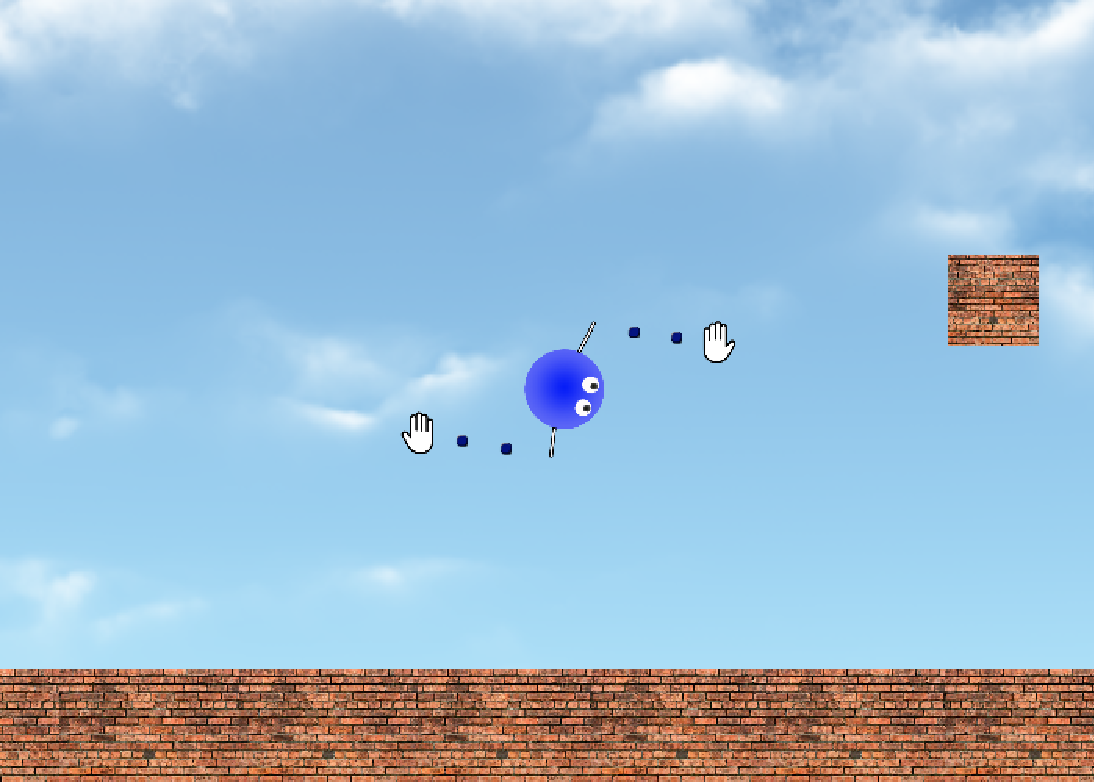
\includegraphics[width=.8\linewidth]{360cropped}
		\caption{Agent performing a Jump 360}
		\label{fig:sub1}
	\end{subfigure}%
	\begin{subfigure}{.5\textwidth}
		\centering
		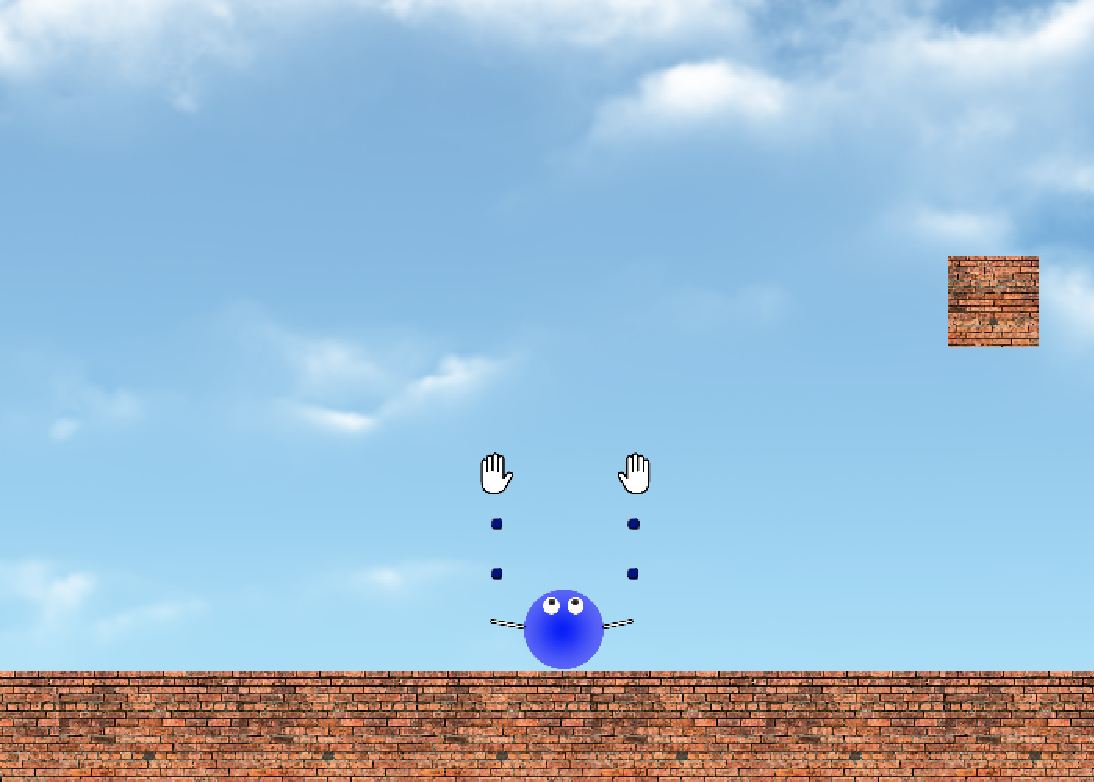
\includegraphics[width=.8\linewidth]{roofcropped}
		\caption{Agent 'raising the roof'}
		\label{fig:sub2}
	\end{subfigure}
	\caption {Agents performing pre-known dance moves}
	\label{fig:dances}
\end{figure}


Table \ref{unlearn} refers to an initial move table.  The top row denotes the current state of the agent, determined by which move the agent performed previously.  The `begin' column indicates the probability that a particular move being the first move of the sequence.  As you can see, the initial probability for any move to be selected as the first dance move is 0.25.  If, for example, move 3 was chosen to be the first move, the agent would then look under the move 3 column to select the next move.  Again, all these probabilities are equal, so the next move will be chosen at random.  The move selection process would continue in this fashion, until the dance to be performed is the correct length.

%INSERT TABLE 1 HERE
\begin{table}[h]
	\begin{center}
		\begin{tabular}{| c | c | c | c | c | c |}
		
		\hline
			 & begin & move 1 & move 2 & move 3 & move 4 \\	\hline	
			move 1 & 0.25 & 0.25 & 0.25 & 0.25 & 0.25 \\	\hline
			move 2 & 0.25 & 0.25 & 0.25 & 0.25 & 0.25 \\	\hline
			move 3 & 0.25 & 0.25 & 0.25 & 0.25 & 0.25 \\	\hline
			move 4 & 0.25 & 0.25 & 0.25 & 0.25 & 0.25 \\	 \hline
		
		\end{tabular} %
	\end{center}
	\caption {Example unlearned move table}
	\label{unlearn}
\end{table}
In order to get the agent to learn a dance, we used a first-order Markov chain.  This allowed the agent to remain essentially memory-less, as `first-order'�� implies that the agent'��s next action is based solely on its current state,�� or in our case, the move that came immediately before.  This could easily be extended to a higher order for more complicated dances or for other desired goals.

If you asked the agent to perform a 4-move dance initially, moves would be selected at random, as each move has an equal probability to be chosen regardless of what state the agent is in.  In order to begin teaching the agent, the user must tell the agent to enter learning mode. Learning mode begins with the agent generating all possible moves for all possible states, using iterative deepening depth first search.  The first moves in this sequence would be single moves; these are used to 'teach' the first move in the desired dance.  After these single moves, the agent would move on to two-move combinations.  The agent would perform a move from the tree, then await feedback from the user.  The user would respond with either `good' or `bad' using the text box built in to PAGI World.  The agent would store this feedback, and then continue on to the next move in the tree.  After the agent received feedback from all possible single moves/move combinations, the agent would begin to generate the new move table.  Each move for a particular state would receive a probability of $1/N$, where $N$ is the number of moves in that state that received positive feedback.  This table would then replace the move table previously in the agent's knowledge.

Table \ref{tab:learn1} demonstrates what the move table could look like after learning has occurred.  As before, the top row indicates the current state of the agent, and the probabilities a move will be chosen for a particular state corresponds to the row labeled accordingly.  In this table, move 2 is the only move that has a chance to be picked as the first move.  From there, the agent will move on to the `move 2' state to select the next move.  In this state, the only move that can be chosen is move 3.  The agent will continue selecting moves in this fashion, until the dance is of the correct length, in this case, a 4 move dance.

%INSERT TABLE 2 HERE
\begin{table}[h]
	\begin{center}
		\begin{tabular}{| c | c | c | c | c | c |}
		
			\hline
			 & begin & move 1 & move 2 & move 3 & move 4 \\	\hline	
			move 1 & 0 & 0 & 0 & 0 & 0 \\	\hline
			move 2 & 1 & 0 & 0 & 0 & 1 \\	\hline
			move 3 & 0 & 1 & 1 & 0 & 0 \\	\hline
			move 4 & 0 & 0 & 0 & 1 & 0 \\	 \hline
		\end{tabular} %
	\end{center}
	\caption {Example learned move table}
	\label{tab:learn1}
\end{table}
Noise can be interjected into the agents move table simply by giving multiple moves within a single state positive feedback.  This would allow $N$ moves to be selected at a single state, provided these $N$ moves were all given `good' as feedback during the learning process.  This would give the agent a little more freedom in the dance that selected.  Feedback given in this manner could allow the agent to perform a `freestyle' dance, while allowing only one move to be selected at a particular state (as in table \ref{tab:learn1}) would call for a specific routine.  Below is an example of a `freestyle' move table.

\begin{table}[h]
	\begin{center}
		\begin{tabular}{| c | c | c | c | c | c |}
			\hline
			 & begin & move 1 & move 2 & move 3 & move 4 \\	\hline	
			move 1 & 0.33 & 0.5 & 0 & 0 & 0.25 \\	\hline
			move 2 & 0.33 & 0 & 0.33 & 0 & 0.25 \\	\hline
			move 3 & 0 & 0.5 & 0.33 & 0 & 0.25 \\	\hline
			move 4 & 0.33 & 0 & 0.33 & 1 & 0.25 \\	 \hline
		
		\end{tabular}  %
	\end{center} 
	\caption{Example learned move table with noise}
	\label{tab:learn2}
\end{table}

Using the tools outlined above, we were able to successfully teach the agent how to dance.  The agent started out with zero knowledge on how to combine his dance moves into a cohesive dance, and after learning the agent could successfully dance any time he was asked.  This simple example demonstrates the simplicity of interacting with an AI agent through verbal�� commands in PAGI World. 
%another task believed to demonstrate animal intelligence...talk about dogs

\subsection{Operant Conditioning Chamber and Classical Conditioning}

There are multiple kinds of learning a successful AGI system can make use of; this environment focuses on Classical Conditioning using a na\"{i}ve Bayesian probability model.

An Operant conditioning chamber (also called a Skinner box) is an apparatus used in the study of animal behavior. %Jack, although these concepts are well-known in psychology, we still need to cite something here. Can you figure out what we need to cite?
Operant conditioning chambers contain at least one operandum (typically a lever) and a means of delivering a primary reinforcer (a reward/punishment pair, e.g. apple/poison). Some operant chambers incorporate lights, sounds and/or drawings to produce multiple stimuli and signify when food is available.

It is easy to construct an operant conditioning chamber in PAGI World. A dispenser is placed within grabbing distance of the agent which when grabbed can produce a primary reinforcer (apples or poison).  These objects have associated positive and negative `endorphins' which the agent can respond to just as an animal would. 


\begin{figure}[h]
\centering
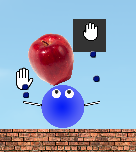
\includegraphics{dispenser}
\caption{PAGI World Operant Conditioning Chamber.} %expand on this caption a little---describe what we're looking at. Same applies to the next figure's caption.
\end{figure}


The application of such an environment is to test classical conditioning algorithms before full scale deployment.  One can limit the number of variables and focus solely on the agent's ability to interpret conditioned stimulus (CS)/unconditioned stimulus (US) pairs.

One such classical conditioning algorithm is implemented using a na\"{i}ve Bayesian probability model. %same here: please find out what a good citation is for this. Wikipedia itself isn't a good source, but it might point you to academic papers that are.
 The agent starts with the assumption that no action of his will lead to endorphins.  Once placed in the operant conditioning chamber, the agent tries to interact with the dispenser.  If this interaction with the dispenser produces endorphins, the CS-US pair is strengthened.  The strength of this CS-US pair is measured as a probability.

The agent is run through a number of tests, each time able to grab the dispenser a set number of times, or for a set period of time.  At the end of each trial, probabilities and the history of the dispenser are saved in a memory file to be used as the initial cases for the next trial.  PAGI World also has built in functions that allow one to change the dispenser's qualities.  This is used to replicate the phenomenon of extinction. %citation for extinction required. An introductory psychology textbook might suffice.


\begin{figure}[h]
\centering
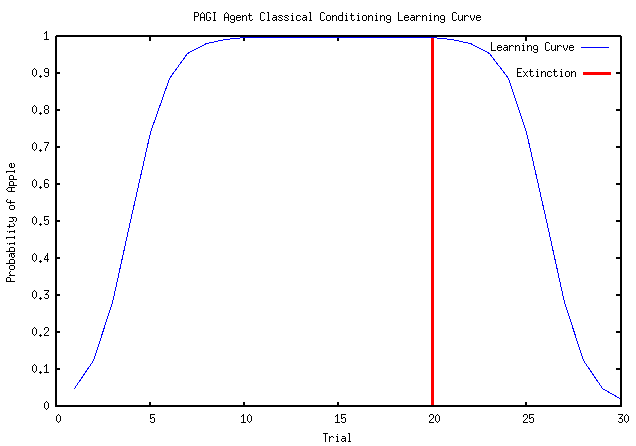
\includegraphics[scale=0.5]{cc_graph}
\caption{Agent Learning Curve}
\end{figure}

In this experiment the agent was provided with a dispenser that produced apples on every grab.  The graph shows the agent coming to this conclusion, as the probability of the dispenser dropping an apple rises to nearly one.  However, after 20 trials the dispenser is turned off.  The conditioned stimulus (grabbing the dispenser) is no longer paired with the conditioned response (endorphin increase due to apple).  Thus, a gradual weakening of the conditioned response can be observed, expressed on the graph as the decrease in the probability of an apple falling.  

This is just one simple example of the flexibility of PAGI World.  Both the operant conditioning chamber and example classical conditioning algorithm could be expanded to be more functional. %in what ways?

%\section{Criticisms}
\label{sect:criticisms}

Although we have tried to be as accommodating as possible, there may still be some concerns and misunderstandings about PAI World and the theory behind it. This section will attempt to address such concerns.

\subsubsection{``PAGI World is not welcoming to top-down AI approaches, or approaches that rely heavily on explicit knowledge."}

It is true that the communication between the agent and the environment is restricted to mostly low-level information. However, this does not mean that the reasoning (or other processes used by the agent) also have to be exclusively low-level. Top-down approaches, such as those in the Logicist AI (LAI) camp \cite{Bringsjord2008c}, can and should benefit from attempts to bridge explicit and implicit knowledge, \textit{but cannot do so if they do not have sufficient access to both types.} 

According to Bringsjord (2008), ``even dynamic perception and action can be systematically logic-based," and thus the exclusively low-level information in PAGI World can spur the development of dynamic perception tools, whether logic-based or not. PAGI World can thus serve as a target for LAI and non-LAI researchers alike---though admittedly they may focus initially on different tasks, we hold that tasks of interest to both schools of thought can be captured in PAGI World. For example, planning of the sort that would be required by the MacGuyver water-directing task described in Section \ref{sect:macgyver} may be difficult to do without symbolic manipulation and reasoning. PAGI World is general enough to allow for tasks that require reasoning over high-level and low-level knowledge alike.

\subsubsection{``PAGI World assumes that embodied cognition is necessary for AGI," or ``conditions \textbf{C1-C3} are simply a restatement of Brooks' (1991) thesis."}

This objection is related to the previous, and just like the previous it is simply not true. PAGI World does not take a position on which approach to modeling cognition is best; rather, it provides an environment in which all approaches should have equal opportunity (as much as possible) to flourish, and therefore gives the field of AI a common benchmark to compare vastly different modeling approaches. A researcher not interested in modeling embodied cognition can focus instead on those tasks on which good performance is predominately determined by higher-level cognitive abilities. 

Guerin (2011) argued that his points, in which \textbf{C1 - C3} are rooted, constituted a weaker form of Brooks's (1991) thesis, in that Guerin only requires that AGI agents be built in a microworld with ``certain essential features of the world," while Brooks requires that no less than the real world be used \cite{Brooks1991}. We do not even take a position that is as strong as Guerin's, at least in this paper. \textit{PAGI World does not assume that bottom-up AI is needed for AGI, it only assumes that AGI must be able to exist in a world in which no more than low-level information is directly available to the AI agent.} The distinction is subtle, admittedly, and it may be the case that the reader already interprets Brooks' or Guerin's theses as equivalent to our own. We do not take a position here that rules out the possibility of AGI being developed outside of an environment like PAGI World, in for example an environment with nothing but logical representations. We do, however, require that AGI be demonstrated to perform well in an environment like PAGI World, on the sort of PAGI tasks that PAGI World specializes in.

\subsubsection{``Eventually all of the tasks are going to be figured out."}

This would be fantastic, because a goal of PAGI World is to encourage the development of artificially-intelligent agents who can solve certain psychometric tasks. AI approaches which are able to solve many of these tasks will have a strong claim to being the currently-best PAGI systems. Furthermore, if there are multiple AI approaches which solve the same tasks, the very fact that they use the same simulation environment will allow us a direct comparison of the alternate AI approaches which is currently lacking from a field that seems like it has a new test environment for every task---this was in fact one of the problem areas identified by Guerin (2011).

What if we run out of interesting tasks? This is where our focus on designing an interface that makes it extremely easy to create new tasks comes in. So long as researchers come up with ideas for how to test AI systems, PAGI World will offer an environment to create tasks to test those ideas. It is requested that any researcher who creates a new task makes that task available to others. We plan on creating a website that will serve as a central repository for all such tasks.

%%%%%%%%%%%%%%%LEFT OFF HERE%%%%%%%%%%%%%%%

\subsubsection{``Certain essential features of physical causality, including detailed vision, sound, etc. are not included."}

Given that this is a simulation environment which strives for realism, and that it is therefore not the same as the real world, at some level a degree of abstraction is unavoidable. These abstractions have already been mostly discussed: finitely sized vectors describing tactile features, 2D rather than 3D physics, etc. 

However, PAGI World offers a framework which future expansions can follow. There is nothing at present preventing PAGI World from simulating sound events and sending low-level sound data to the agent just as it does with visual and tactile data. We have simply chosen not to prioritize the development of a realistic sound simulator at this time.

\subsubsection{``A lot of learning children do is by example, which PAGI World doesn't support."}

This is simply not true. We support at least two forms of supervised instruction: There is an input text box through which human users can type and send strings directly to the AI script, which can serve as feedback. This form of instruction is used in the dancing task we described earlier in this paper. Secondly, the endorphin system, also mentioned earlier, which allows certain foods to be rewards and others to be negative stimuli, can also be used as a method of training AI systems.

Furthermore, we are currently developing a component that will allow for a second AI agent to exist simultaneously in a task. Details for the most effective way to implement this are still being considered, and we welcome suggestions from the readers and any researchers who use the beta version of PAGI World.


%\section{Conclusion and Future Work}

The release of PAGI World is accompanied with a call to all AGI and human-level-AI researchers to finally examine the strengths and limits of their preferred approaches. PAGI World allows for researchers to very easily create tasks and microworlds in a 2D world with realistic physics, with no knowledge in how to program. PAGI World can interact with AI agents that are written in virtually any programming language, and the simulation can be run on any major operating system. We have very carefully designed PAGI World to have an extremely low technical barrier, so that many researchers can find common ground upon which to compare their different approaches.

The future of PAGI World is bright. We already have several AI systems in progress whose goals are to solve already-finished PAGI World tasks, and as development continues we hope to greatly increase the number of tasks which are available and the sophistication of the agents which solve those tasks. The library of future tasks, we hope, will diversify and reflect the broad spectrum of tasks which require human-like intelligence. 

One interesting and possibly fertile source of PAGI World tasks is the area of morality. Figure \ref{FIGURE_MORALITY} depicts an example task in which two food objects---an apple and a piece of bacon---are falling down a series of ramps where they will eventually fall off the screen and become unreachable, unless the agent chooses exactly one of them (he will not be able to get both in time). Although not many would consider the choice between apples and bacon to be a moral decision, it is easy to see how such a scenario can be adapted to capture miniature moral dilemmas. For example, if the simulation begins with the agent having knowledge that an apple will save the life of person \textbf{A}, while the bacon will save person \textbf{B} but leave \textbf{A} to die, suddenly Figure (FIG) becomes a moral decision which the agent must make in real time. Examples like these illustrate the wide variety of tasks and demonstrations that can be created with PAGI World.

Special thanks to Kainoa Eastlack for helping us with an earlier version of PAGI World.

This work was supported in part by 



\bibliographystyle{acm}
\bibliography{john}

\end{document}

